\section{Fill models against real outcomes}
\label{sec:fillmodels}

\subsection{Design}
Each model is asked one question about each real order: \emph{would it have been
filled within the time the order actually lived}, that is, before its real
first fill, its cancellation or the end of observation? A model sees only the
market around the order---trades at its price and the queue ahead---never the
order's own fills. Because the true outcome of every order is known, the error
of each fill assumption is measured separately from any strategy. Orders placed
in the first five minutes of a cold-started hour are excluded.

\subsection{Models}
Trades are aggregated by block and price level, the block being the smallest
unit of time the data distinguishes; a trade hits the side opposite its
aggressor.
\begin{description}
  \item[\touch.] The first trade at the order's price fills it.
  \item[\vt.] The first trade after which the volume traded at the order's price
  since placement exceeds the volume ahead at placement fills it. Cancellations
  ahead are invisible to it.
  \item[\qa.] The first trade at the order's price after the order has reached
  the front of its queue fills it.
  \item[\clock.] Fills arrive with intensity $\lambda(\delta)=A e^{-k\delta}$,
  where $\delta$ is the distance from the mid-price before placement in ticks;
  the model's answer is the probability of at least one fill during the order's
  life. $A$ and $k$ are fitted per hour from the farthest level each block's
  trading reached, by a log-linear fit weighted by count (and, for comparison,
  unweighted).
\end{description}

\subsection{Results}

\begin{table*}[t]
\centering\small
\caption{Four fill rules against the real outcomes of passive orders, pilot
hour (518\,409 \SOL{} and 1\,610\,840 \BTC{} orders). ``$\times$ real'' is the
model's fill rate over the observed one. False fills are a share of unfilled
orders; missed fills a share of filled ones.}
\label{tab:fillmodels}
\begin{tabular}{@{}l rrrr c rrrr@{}}
\toprule
 & \multicolumn{4}{c}{\SOL} && \multicolumn{4}{c}{\BTC} \\
\cmidrule{2-5}\cmidrule{7-10}
Rule & filled & $\times$ real & false & missed && filled & $\times$ real & false & missed \\
\midrule
Observed           & 0.85\% & 1     & --     & --      && 1.61\% & 1     & --     & --      \\
\touch             & 5.16\% & 6.07  & 4.34\% & 0.05\%  && 7.57\% & 4.71  & 6.06\% & 0.00\%  \\
\vt                & 0.29\% & 0.34  & 0.02\% & 68.60\% && 0.76\% & 0.47  & 0.04\% & 55.26\% \\
\qa                & 0.89\% & 1.05  & 0.04\% & 0.09\%  && 1.65\% & 1.02  & 0.04\% & 0.13\%  \\
\clock, weighted   & 8.70\% & 10.23 & \multicolumn{2}{c}{probability} && 9.91\% & 6.16 & \multicolumn{2}{c}{probability} \\
\clock, unweighted & 6.16\% & 7.25  & \multicolumn{2}{c}{probability} && 2.85\% & 1.78 & \multicolumn{2}{c}{probability} \\
\bottomrule
\end{tabular}
\end{table*}

\begin{figure*}[t]
\centering
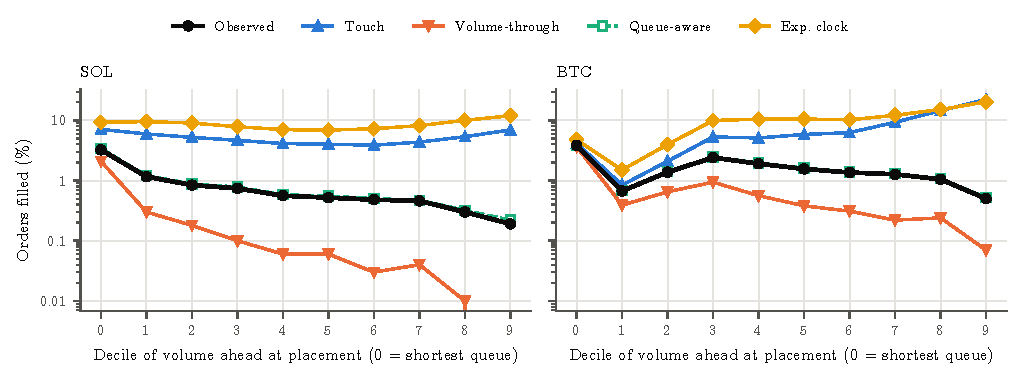
\includegraphics[width=\textwidth]{fill_by_decile}
\caption{Share of orders filled, by decile of the volume resting ahead at
placement: observed, and according to each fill rule (log scale). Pilot hour,
orders placed after the five-minute warm-up. \vt{} gives no fill at all in the
last \SOL{} decile, which the log scale cannot show.}
\label{fig:deciles}
\end{figure*}

Table~\ref{tab:fillmodels} gives the results and Figure~\ref{fig:deciles}
breaks them down by queue position.

\paragraph{\touch{} overstates fills five- to six-fold} and misses almost none:
every real fill is preceded by a touch. Its error grows with queue depth: in the
last decile of volume ahead on \BTC{} it predicts 22.19\% against a real 0.50\%,
44 times too many. The rule does not merely shift the level of fills; it inverts
their dependence on queue position, the very dependence on which a market
maker's decisions rest.

\paragraph{\vt{} understates fills two- to three-fold} and misses 69\% (\SOL) and
55\% (\BTC) of real fills. The cause is measured directly: of the volume ahead of
orders that reached the front, \textbf{98.2\% (\SOL) and 94.5\% (\BTC) left by
cancellation}, not by trading. The rule waits for volume to trade away that is in
fact almost entirely withdrawn. Its caution is not conservative: it errs in the
other direction by a comparable factor.

\paragraph{\qa{} reproduces the observed rate to within 5\%} on both instruments
and follows the observed dependence on queue position in every decile. Its one
systematic error is the subject of Section~\ref{sec:block}: of its 217 false
fills on \SOL{} and 667 on \BTC, 201 and 625 fall on a trade in the very block in
which the order was cancelled. Of its missed fills (4 and 33), 2 and 32 are the
matching-time removals of Section~\ref{sec:outcomes}.

\begin{figure}[t]
\centering
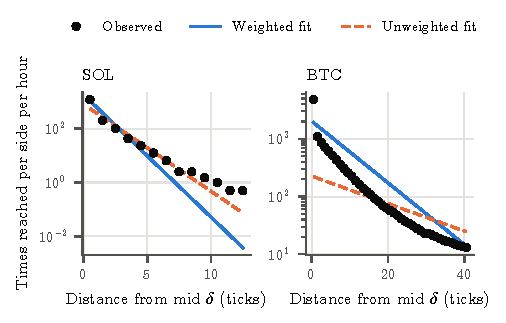
\includegraphics[width=\columnwidth]{clock_fit}
\caption{How often trading reaches $\delta$ ticks from the mid-price, per side
per hour, against the exponential intensity fitted with and without weights
(log scale). Pilot hour; \BTC{} truncated at 40 ticks.}
\label{fig:clock}
\end{figure}

\paragraph{\clock{} is governed by its calibration.} Two equally defensible fits
give an excess of 10.2 or 7.3 times on \SOL{} and of 6.2 or 1.8 times on \BTC.
The exponential form does not fit (Figure~\ref{fig:clock}): trading reaches half a tick from the mid
4\,791 times per side per hour on \BTC, against 1\,914 for the weighted fit and
220 for the unweighted one, and the tail is heavy (from 1.5 to 2.5 ticks the
count falls only from 1\,096 to 868). Like \touch, the clock ignores the queue;
across deciles its answer rises with queue depth on \BTC{} from 4.8\% to 20.3\%
while the real rate falls.

\subsection{One cause, two errors}
The two standard event rules err in opposite directions, and for one reason:
cancellations ahead in the queue. \touch{} ignores the queue entirely;
\vt{} sees it, but sees it drain only through trades. A rule that tracks the
queue reproduces the facts, but it requires the stream of book changes with
order identities---data at the L4 level.

